\documentclass{standalone}
\usepackage{tikz}
\usetikzlibrary{patterns, positioning}


\begin{document}
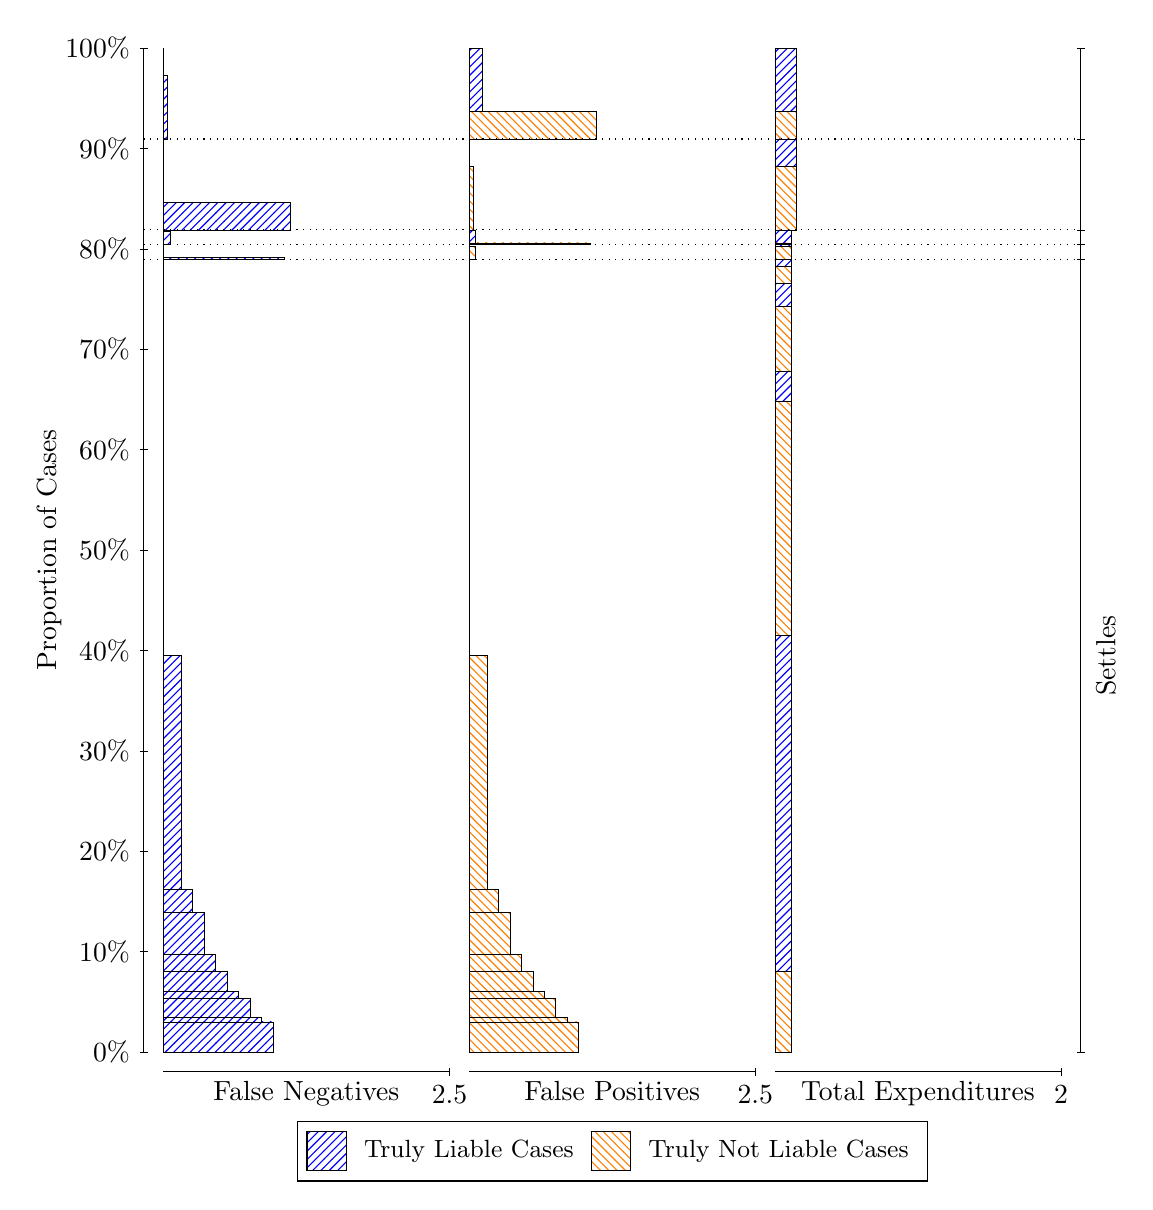
\begin{tikzpicture}
\draw[black, very thin] (1.5,1.75) -- (1.5,14.5);
\node[rotate=90, text=black, anchor=center] at (0.3, 8.125) {Proportion of Cases};
\draw[black, very thin] (1.45,1.75) -- (1.55,1.75);
\node[text=black, anchor=east] at (1.45, 1.75) {0\%};
\draw[black, very thin] (1.45,3.025) -- (1.55,3.025);
\node[text=black, anchor=east] at (1.45, 3.025) {10\%};
\draw[black, very thin] (1.45,4.3) -- (1.55,4.3);
\node[text=black, anchor=east] at (1.45, 4.3) {20\%};
\draw[black, very thin] (1.45,5.575) -- (1.55,5.575);
\node[text=black, anchor=east] at (1.45, 5.575) {30\%};
\draw[black, very thin] (1.45,6.85) -- (1.55,6.85);
\node[text=black, anchor=east] at (1.45, 6.85) {40\%};
\draw[black, very thin] (1.45,8.125) -- (1.55,8.125);
\node[text=black, anchor=east] at (1.45, 8.125) {50\%};
\draw[black, very thin] (1.45,9.4) -- (1.55,9.4);
\node[text=black, anchor=east] at (1.45, 9.4) {60\%};
\draw[black, very thin] (1.45,10.675) -- (1.55,10.675);
\node[text=black, anchor=east] at (1.45, 10.675) {70\%};
\draw[black, very thin] (1.45,11.95) -- (1.55,11.95);
\node[text=black, anchor=east] at (1.45, 11.95) {80\%};
\draw[black, very thin] (1.45,13.225) -- (1.55,13.225);
\node[text=black, anchor=east] at (1.45, 13.225) {90\%};
\draw[black, very thin] (1.45,14.5) -- (1.55,14.5);
\node[text=black, anchor=east] at (1.45, 14.5) {100\%};

\draw[black, very thin] (13.4,1.75) -- (13.4,14.5);
\draw[black, very thin] (13.35,1.75) -- (13.45,1.75);
\node[anchor=west] at (13.35, 1.75) {};
\draw[black, very thin] (13.35,11.817) -- (13.45,11.817);
\node[anchor=west] at (13.35, 11.817) {};
\draw[black, very thin] (13.35,12.003) -- (13.45,12.003);
\node[anchor=west] at (13.35, 12.003) {};
\draw[black, very thin] (13.35,12.19) -- (13.45,12.19);
\node[anchor=west] at (13.35, 12.19) {};
\draw[black, very thin] (13.35,13.345) -- (13.45,13.345);
\node[anchor=west] at (13.35, 13.345) {};
\draw[black, very thin] (13.35,14.5) -- (13.45,14.5);
\node[anchor=west] at (13.35, 14.5) {};

\draw[black, very thin, pattern color=blue, pattern=north east lines] (1.75,1.75) rectangle (3.1398,2.1314);
\draw[black, very thin, pattern color=blue, pattern=north east lines] (1.75,2.1314) rectangle (2.9944,2.1846);
\draw[black, very thin, pattern color=blue, pattern=north east lines] (1.75,2.1846) rectangle (2.8491,2.4267);
\draw[black, very thin, pattern color=blue, pattern=north east lines] (1.75,2.4267) rectangle (2.7037,2.5188);
\draw[black, very thin, pattern color=blue, pattern=north east lines] (1.75,2.5188) rectangle (2.5584,2.7771);
\draw[black, very thin, pattern color=blue, pattern=north east lines] (1.75,2.7771) rectangle (2.4131,2.9896);
\draw[black, very thin, pattern color=blue, pattern=north east lines] (1.75,2.9896) rectangle (2.2678,3.5186);
\draw[black, very thin, pattern color=blue, pattern=north east lines] (1.75,3.5186) rectangle (2.1224,3.8154);
\draw[black, very thin, pattern color=blue, pattern=north east lines] (1.75,3.8154) rectangle (1.9771,6.7833);
\draw[black, very thin, pattern color=orange, pattern=north west lines] (1.75,6.7833) rectangle (1.75,11.817);
\draw[black, very thin, pattern color=blue, pattern=north east lines] (1.75,11.817) rectangle (3.2851,11.837);
\draw[black, very thin, pattern color=orange, pattern=north west lines] (1.75,11.837) rectangle (1.75,12.003);
\draw[black, very thin, pattern color=blue, pattern=north east lines] (1.75,12.003) rectangle (1.8318,12.169);
\draw[black, very thin, pattern color=orange, pattern=north west lines] (1.75,12.169) rectangle (1.75,12.19);
\draw[black, very thin, pattern color=blue, pattern=north east lines] (1.75,12.19) rectangle (3.3668,12.541);
\draw[black, very thin, pattern color=orange, pattern=north west lines] (1.75,12.541) rectangle (1.75,13.345);
\draw[black, very thin, pattern color=blue, pattern=north east lines] (1.75,13.345) rectangle (1.8045,14.149);
\draw[black, very thin, pattern color=orange, pattern=north west lines] (1.75,14.149) rectangle (1.75,14.5);
\draw[black, very thin, pattern color=orange, pattern=north west lines] (5.6333,1.75) rectangle (7.0231,2.1314);
\draw[black, very thin, pattern color=orange, pattern=north west lines] (5.6333,2.1314) rectangle (6.8777,2.1846);
\draw[black, very thin, pattern color=orange, pattern=north west lines] (5.6333,2.1846) rectangle (6.7324,2.4267);
\draw[black, very thin, pattern color=orange, pattern=north west lines] (5.6333,2.4267) rectangle (6.5871,2.5188);
\draw[black, very thin, pattern color=orange, pattern=north west lines] (5.6333,2.5188) rectangle (6.4417,2.777);
\draw[black, very thin, pattern color=orange, pattern=north west lines] (5.6333,2.777) rectangle (6.2964,2.9896);
\draw[black, very thin, pattern color=orange, pattern=north west lines] (5.6333,2.9896) rectangle (6.1511,3.5186);
\draw[black, very thin, pattern color=orange, pattern=north west lines] (5.6333,3.5186) rectangle (6.0057,3.8155);
\draw[black, very thin, pattern color=orange, pattern=north west lines] (5.6333,3.8155) rectangle (5.8604,6.7834);
\draw[black, very thin, pattern color=blue, pattern=north east lines] (5.6333,6.7834) rectangle (5.6333,11.817);
\draw[black, very thin, pattern color=orange, pattern=north west lines] (5.6333,11.817) rectangle (5.7151,11.983);
\draw[black, very thin, pattern color=blue, pattern=north east lines] (5.6333,11.983) rectangle (5.6333,12.003);
\draw[black, very thin, pattern color=orange, pattern=north west lines] (5.6333,12.003) rectangle (7.1684,12.024);
\draw[black, very thin, pattern color=blue, pattern=north east lines] (5.6333,12.024) rectangle (5.7151,12.19);
\draw[black, very thin, pattern color=orange, pattern=north west lines] (5.6333,12.19) rectangle (5.6878,12.994);
\draw[black, very thin, pattern color=blue, pattern=north east lines] (5.6333,12.994) rectangle (5.6333,13.345);
\draw[black, very thin, pattern color=orange, pattern=north west lines] (5.6333,13.345) rectangle (7.2502,13.696);
\draw[black, very thin, pattern color=blue, pattern=north east lines] (5.6333,13.696) rectangle (5.7968,14.5);
\draw[black, very thin, pattern color=orange, pattern=north west lines] (9.5167,1.75) rectangle (9.721,2.777);
\draw[black, very thin, pattern color=blue, pattern=north east lines] (9.5167,2.777) rectangle (9.721,7.0416);
\draw[black, very thin, pattern color=orange, pattern=north west lines] (9.5167,7.0416) rectangle (9.721,10.01);
\draw[black, very thin, pattern color=blue, pattern=north east lines] (9.5167,10.01) rectangle (9.721,10.391);
\draw[black, very thin, pattern color=orange, pattern=north west lines] (9.5167,10.391) rectangle (9.721,11.217);
\draw[black, very thin, pattern color=blue, pattern=north east lines] (9.5167,11.217) rectangle (9.721,11.512);
\draw[black, very thin, pattern color=orange, pattern=north west lines] (9.5167,11.512) rectangle (9.721,11.725);
\draw[black, very thin, pattern color=blue, pattern=north east lines] (9.5167,11.725) rectangle (9.721,11.817);
\draw[black, very thin, pattern color=orange, pattern=north west lines] (9.5167,11.817) rectangle (9.721,11.983);
\draw[black, very thin, pattern color=blue, pattern=north east lines] (9.5167,11.983) rectangle (9.721,12.003);
\draw[black, very thin, pattern color=orange, pattern=north west lines] (9.5167,12.003) rectangle (9.721,12.024);
\draw[black, very thin, pattern color=blue, pattern=north east lines] (9.5167,12.024) rectangle (9.721,12.19);
\draw[black, very thin, pattern color=orange, pattern=north west lines] (9.5167,12.19) rectangle (9.7892,12.994);
\draw[black, very thin, pattern color=blue, pattern=north east lines] (9.5167,12.994) rectangle (9.7892,13.345);
\draw[black, very thin, pattern color=orange, pattern=north west lines] (9.5167,13.345) rectangle (9.7892,13.696);
\draw[black, very thin, pattern color=blue, pattern=north east lines] (9.5167,13.696) rectangle (9.7892,14.5);
\draw[black, dotted] (1.5,11.817) -- (13.4,11.817);
\draw[black, dotted] (1.5,12.003) -- (13.4,12.003);
\draw[black, dotted] (1.5,12.19) -- (13.4,12.19);
\draw[black, dotted] (1.5,13.345) -- (13.4,13.345);
\draw[black, very thin] (1.75,1.5) -- (5.3833,1.5);
\node[text=black, anchor=north] at (3.5667, 1.5) {False Negatives};
\draw[black, very thin] (5.3833,1.45) -- (5.3833,1.55);
\node[text=black, anchor=north] at (5.3833, 1.45) {2.5};

\draw[black, very thin] (5.6333,1.5) -- (9.2667,1.5);
\node[text=black, anchor=north] at (7.45, 1.5) {False Positives};
\draw[black, very thin] (9.2667,1.45) -- (9.2667,1.55);
\node[text=black, anchor=north] at (9.2667, 1.45) {2.5};

\draw[black, very thin] (9.5167,1.5) -- (13.15,1.5);
\node[text=black, anchor=north] at (11.333, 1.5) {Total Expenditures};
\draw[black, very thin] (13.15,1.45) -- (13.15,1.55);
\node[text=black, anchor=north] at (13.15, 1.45) {2};

\node[text=black, centered, rotate=90] at (13.72, 6.7834) {Settles};





\draw (7.449999999999999,1.5) node[draw=none] (baseCoordinate) {};
\begin{scope}[align=center]
        \matrix[scale=0.5, draw=black, below=0.5cm of baseCoordinate, nodes={draw}, column sep=0.1cm]{
            \node[rectangle, draw, minimum width=0.5cm, minimum height=0.5cm, pattern color=blue, pattern=north east lines] {}; &
            \node[draw=none, font=\small, text=black] (B) {Truly Liable Cases}; &
            \node[rectangle, draw, minimum width=0.5cm, minimum height=0.5cm, pattern color=orange, pattern=north west lines] {}; &
            \node[draw=none, font=\small, text=black] (B) {Truly Not Liable Cases}; \\
            };
\end{scope}

\end{tikzpicture}
\end{document}